\section{Additional diagnostics of the London chains}
\label{app:london-extra}

This appendix collects the diagnostics of the London chains that Tables~\ref{tab:multistart} and~\ref{tab:las-sens} do not show.

\paragraph{Agreement of the readouts across chains.}
The readouts of Section~\ref{sec:las-structure} are computed per chain before pooling. The share of plans in which a given station is open differs between two chains by at most $0.08$ (mean absolute difference $0.02$ over stations), the share in which two open stations share a Group by at most $0.11$ (mean $0.003$ over pairs), and the contestedness of the LSOAs correlates at $0.96$ or better between any two chains. The Monte Carlo standard error of a station's open frequency, estimated from the four chains, is at most $0.016$, and $0.007$ for the median station. Effective sample sizes per chain range from about $400$ for the cut-edge count and the station-leg energy, the two slowest observables, to $2{,}200$ to $3{,}400$ for the number of Groups.

\begin{figure}[!htbp]
\centering
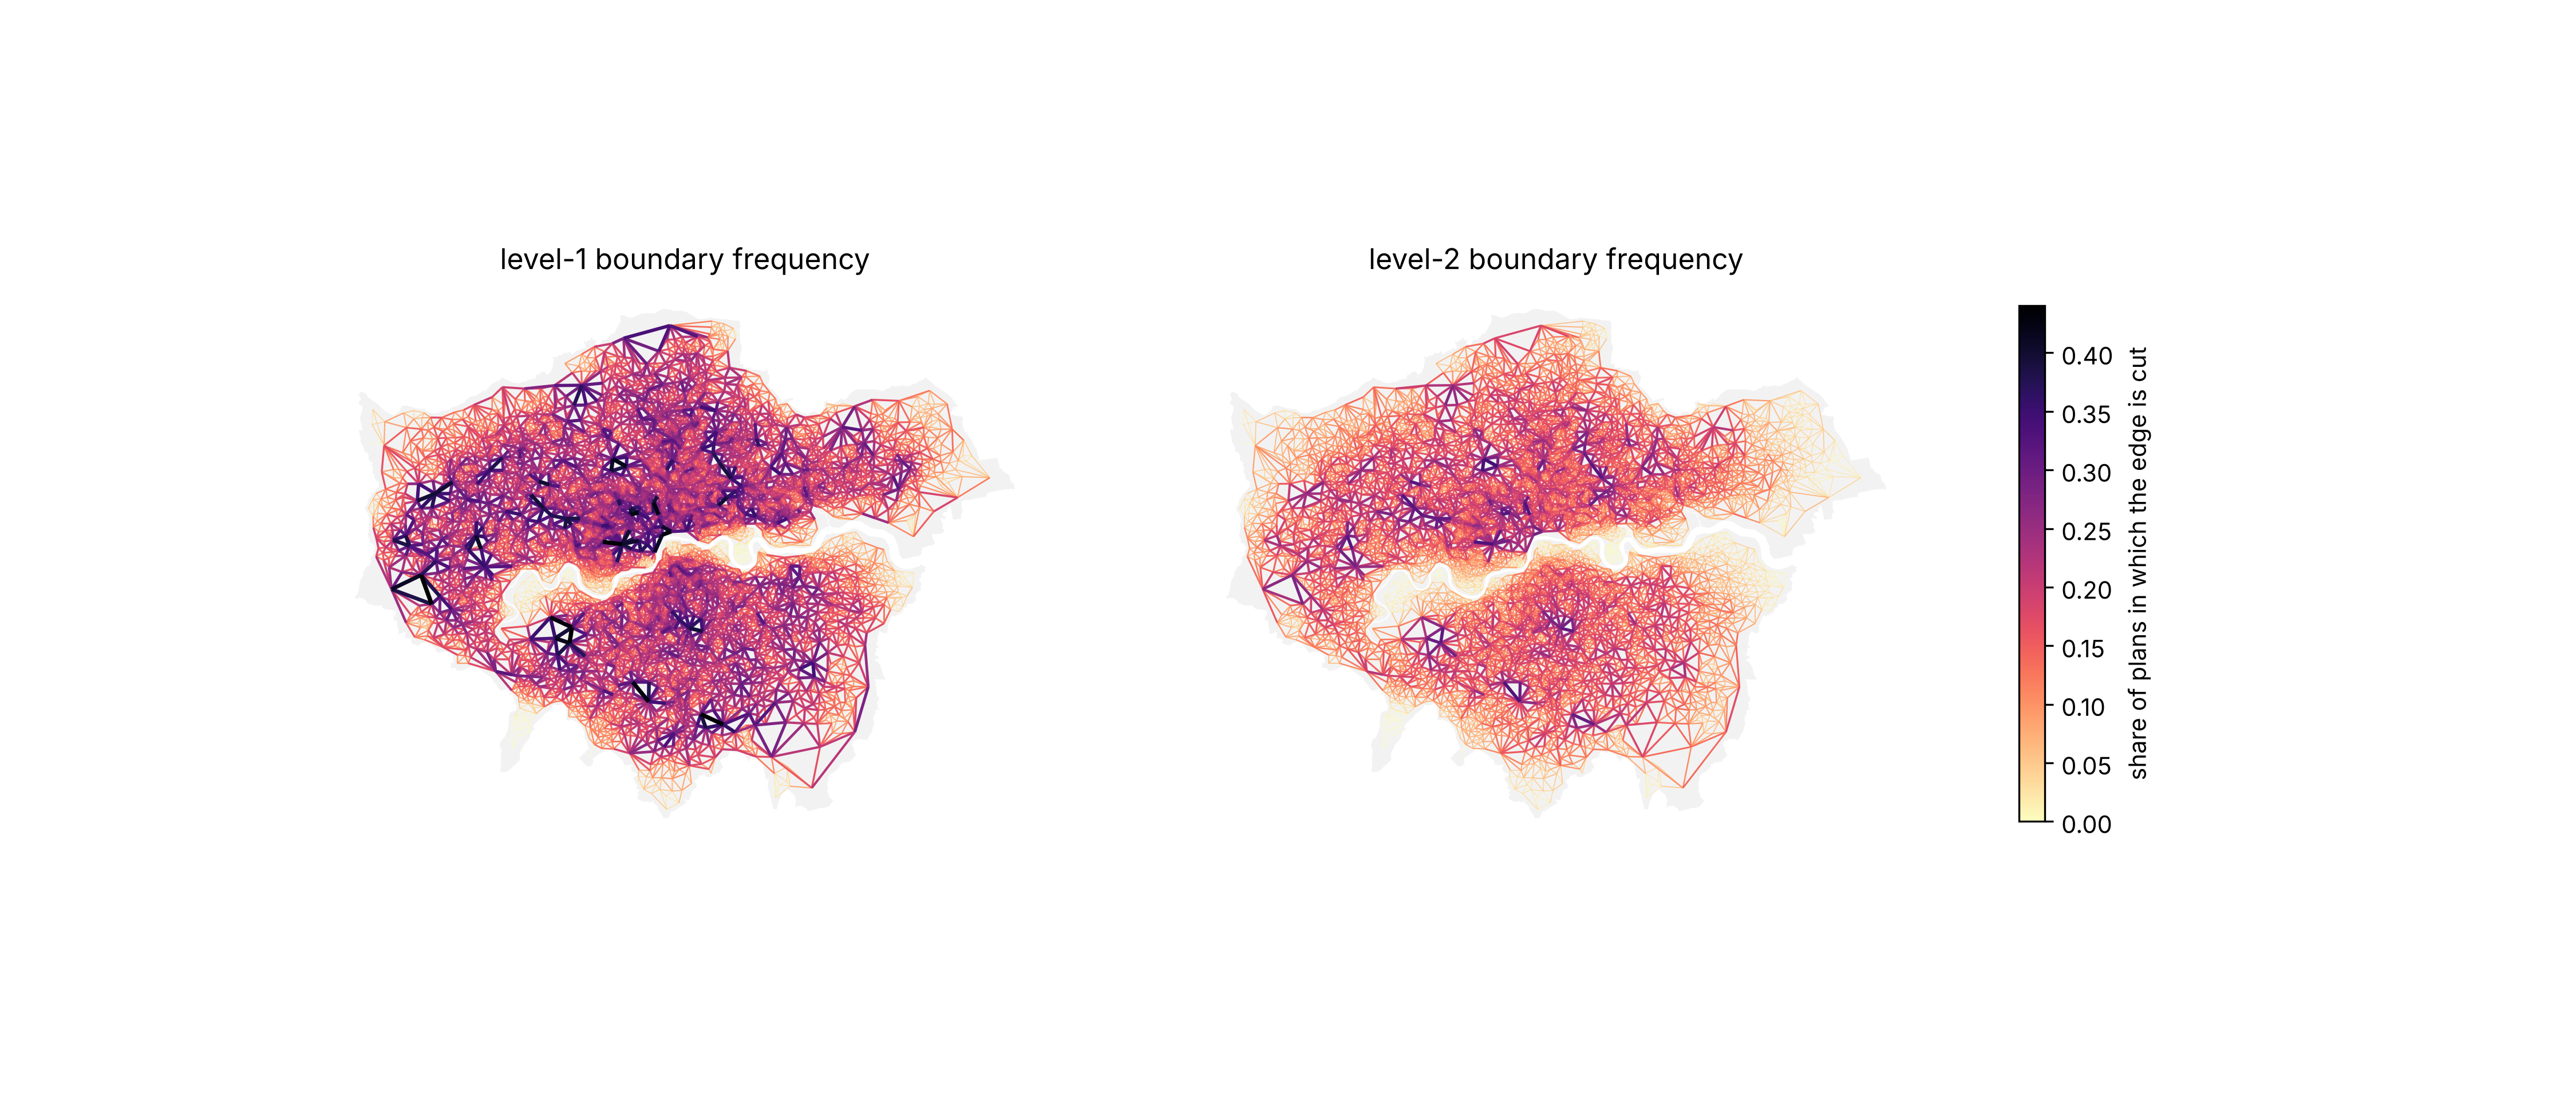
\includegraphics[width=\linewidth,trim=0 80 0 80,clip]{figures/las/fig_boundary_freq.png}
\caption{Share of plans in which each edge of $G^1$ is cut by a station boundary (left) or a Group boundary (right). Darker and thicker edges are cut more often, and the colour scale runs to the largest observed frequency.}
\label{fig:las-boundary}
\end{figure}

\paragraph{Holding times and the law of the accepted moves.}
Holding the state on rejection reweights the sampled law by the expected holding time, $1/a(s)$ for a state $s$ from which a proposal closes with probability $a(s)$ (Section~\ref{sec:convergence-status}). On this instance $a(s)$ is not constant. Pooling the post-burn-in steps, acceptance rises from $0.61$ in states with $46$ open stations to $0.73$ in states with $58$, because a plan with fewer and larger supernodes is harder to re-partition, so the expected holding time falls from $1.64$ steps to $1.37$ and the time law tilts toward plans with fewer open stations; the rejection probability is $0.334$ after a rejected step against $0.315$ after an accepted one. The tilt is small in its effects. Weighting each stored plan by the inverse length of the visit it belongs to, which recovers the law of the jump chain, moves the mean number of open stations from $52.48$ to $52.54$, the capacity shares by at most $0.002$ and the open frequency of any station by at most $0.008$ (mean $0.002$); one station at the threshold, Chiswick, moves from $0.894$ to $0.900$ and joins the set open in more than $90\%$ of plans. We report the time law, which is what the chain samples, and note that the retry budget $M$ enters it through $a(s)$.

\paragraph{The chain from the Group-based start.}
The station-level readouts of the fifth chain of Section~\ref{sec:exp-multistart} agree with those of the four sector-start chains. Its open frequencies differ from the pooled four by at most $0.05$ (mean $0.015$), against $0.045$ for any one of the four on its own. Its set of stations open in more than $90\%$ of plans differs from theirs by five stations whose frequencies lie between $0.89$ and $0.92$ on one side or the other, as each of the four chains on its own differs from the pooled set by two to six such stations. Its mean total energy $E_1+E_2$, $9.69$ million, number of open stations, $52.4$, and adjusted Rand index against the real Groups, $0.28$, lie within the ranges of the four ($9.67$ to $9.69$ million, $52.4$ to $52.6$, $0.27$ to $0.28$).

\begin{figure}[!htbp]
\centering
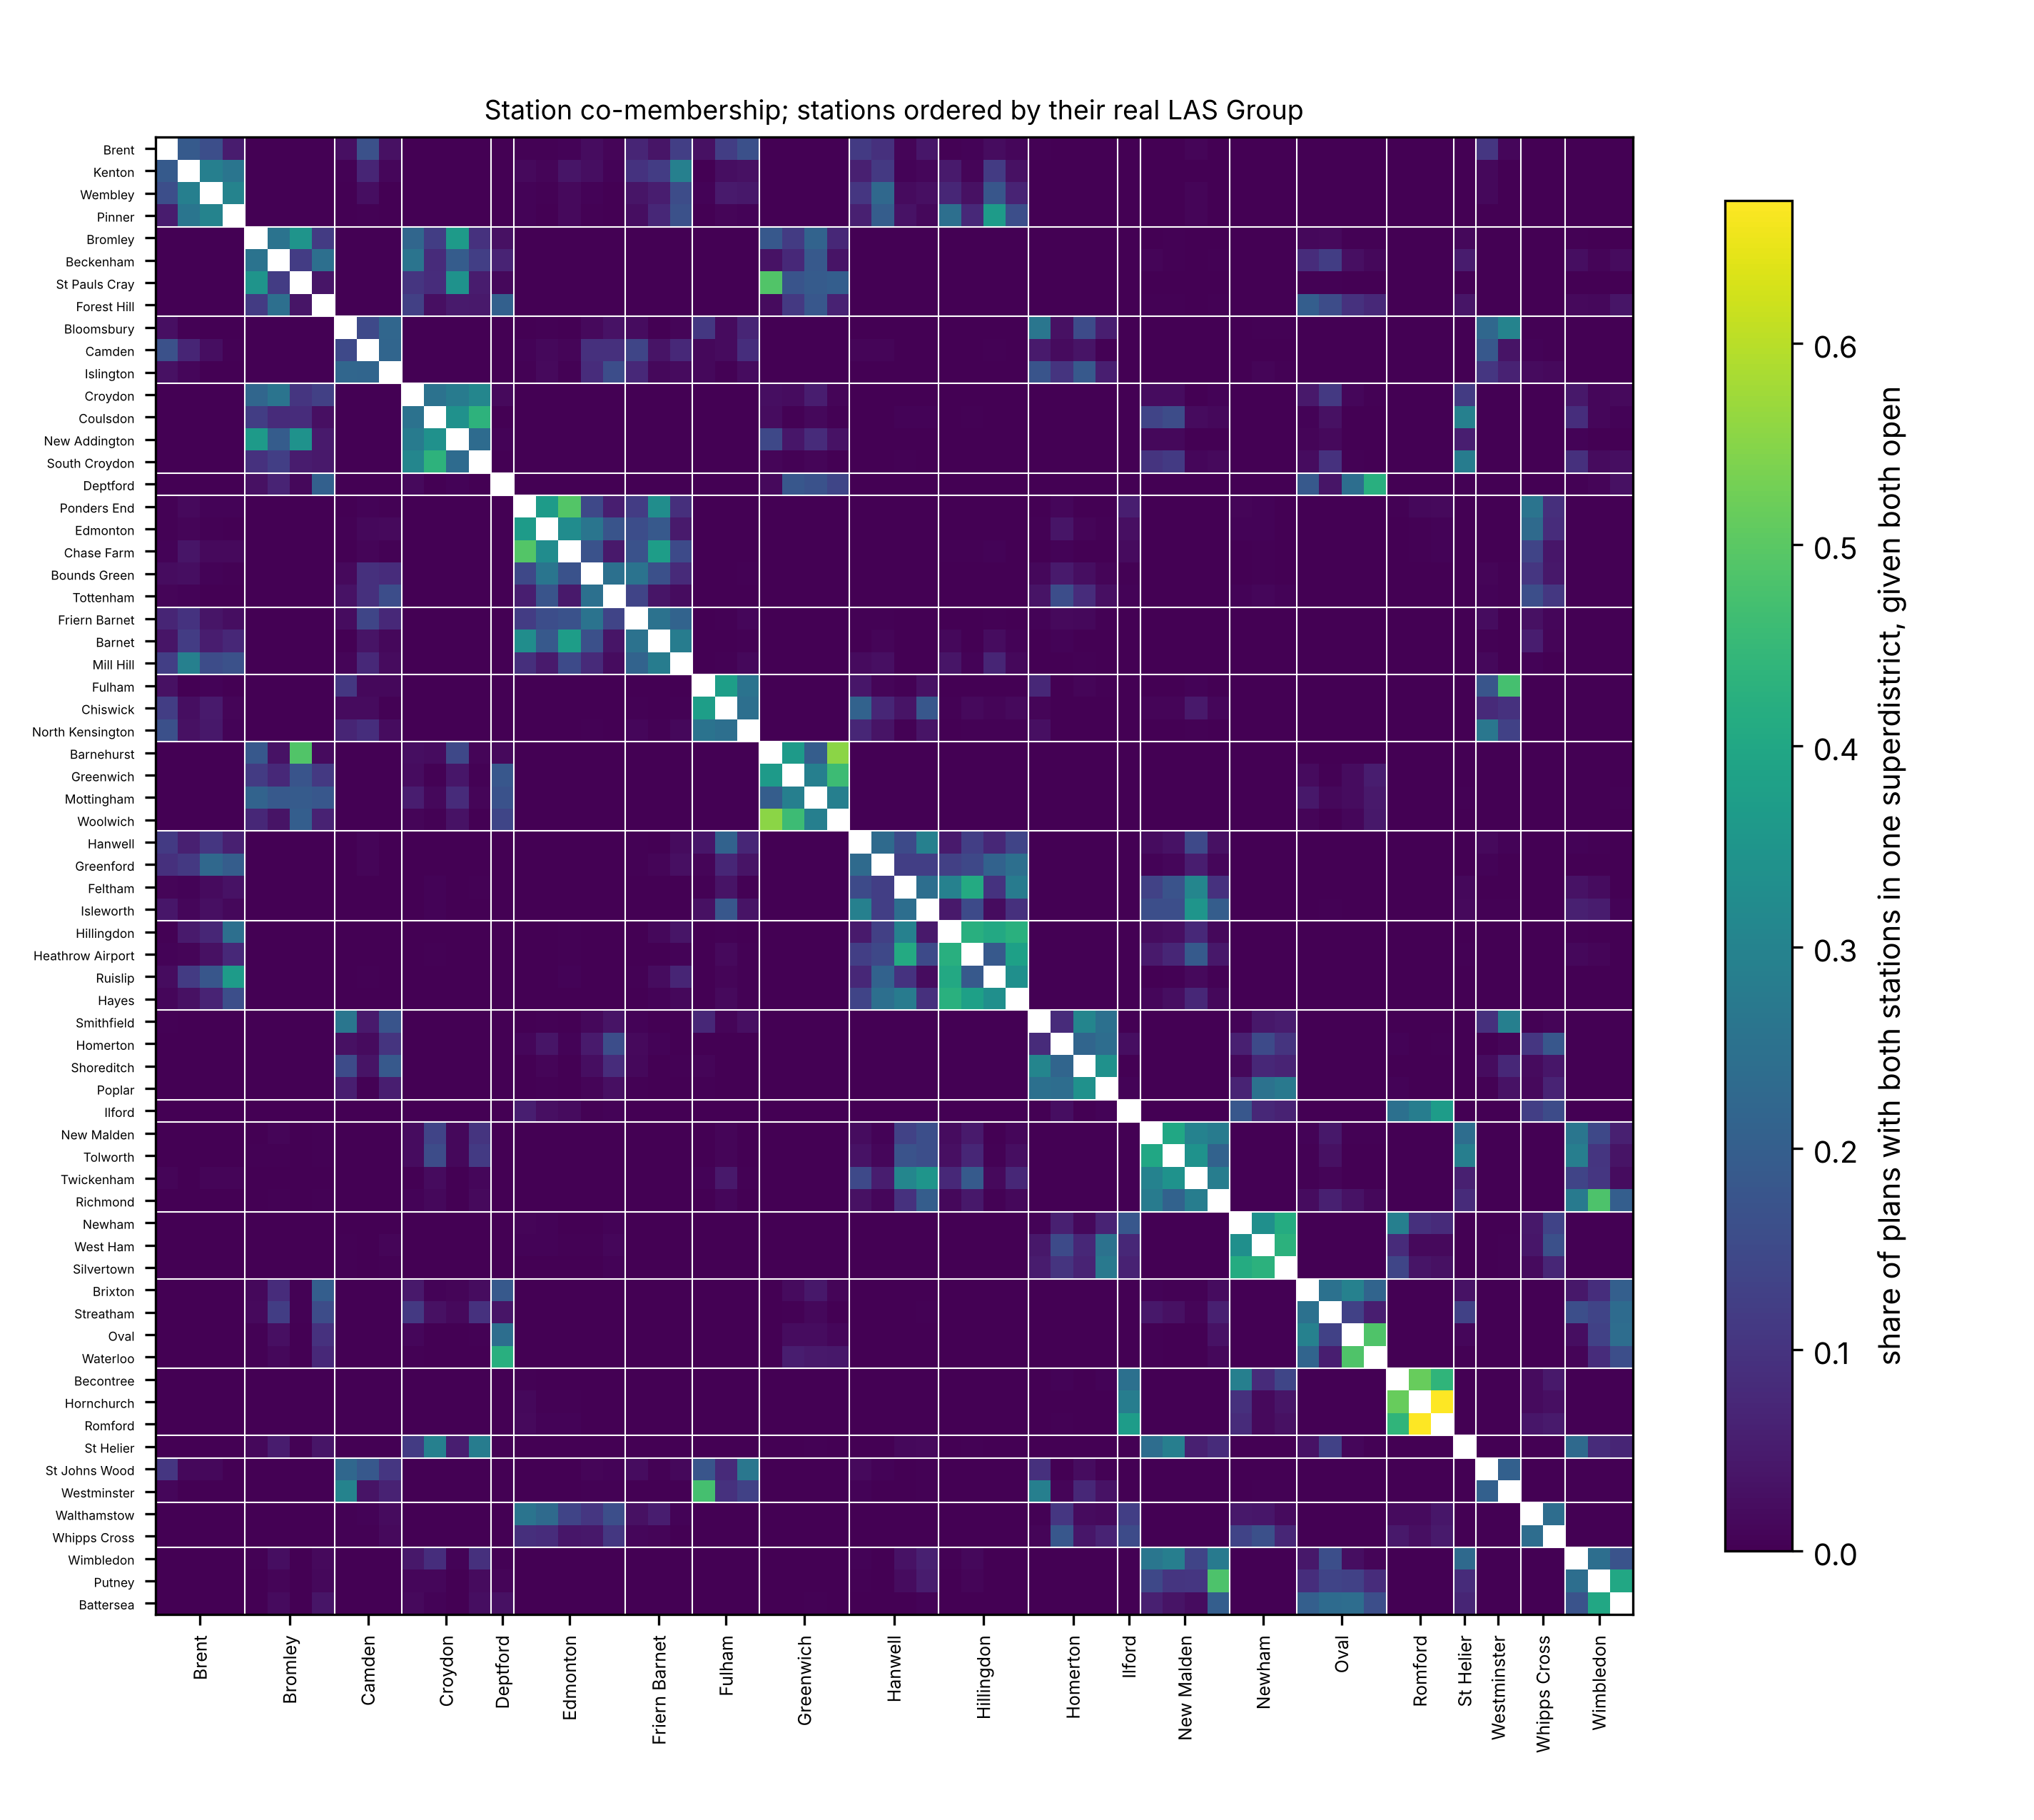
\includegraphics[width=0.52\linewidth]{figures/las/fig_groups.png}
\caption{Share of plans in which two stations belong to the same superdistrict, among the plans in which both are open; stations ordered by their real Group, with white lines separating the $21$ Groups and the colour scale running to the largest off-diagonal value.}
\label{fig:las-groups}
\end{figure}

\paragraph{The two replications.}
Table~\ref{tab:las-sens} reports the replications of Section~\ref{sec:las-sensitivity}. Under the uniform demand proxy the set of stations open in more than $90\%$ of plans exchanges five stations that lie within $0.03$ of the threshold under one proxy or the other: Newham, Ponders End and South Croydon leave, and Chiswick and Tottenham join. The run at tolerance $0.25$ is half as long as the baseline and its diagnostics are correspondingly weaker: split-$\hat R$ is at most $1.008$, the effective sample sizes per chain are $252$ to $438$ for the energy and $145$ to $285$ for the cut-edge count, so that the $3{,}200$ stored plans are worth about $1{,}390$ and $800$ independent draws, and three of the four initial plans needed two attempts.

\paragraph{Station and Group pairs in full.}
Stations open in more than $90\%$ of plans are led by Fulham ($97\%$), St John's Wood ($96\%$), Ilford, Deptford and Barnehurst ($94\%$ each) and Whipps Cross ($93\%$); the least used are Chase Farm ($40\%$), Heathrow Airport ($41\%$), Twickenham ($49\%$), New Addington and Wembley ($60\%$), and Tolworth, Barnet and Richmond ($61\%$). Inner stations such as St John's Wood, Ilford, Camden, Deptford and Brent carry three units in $37\%$ to $42\%$ of the plans in which they are open, and outer stations such as Tolworth, Richmond, Chase Farm, Heathrow Airport and New Addington carry one unit in $67\%$ to $77\%$ of theirs. The pairs kept together most often inside a real Group are Hornchurch and Romford ($67\%$), Barnehurst and Woolwich ($55\%$), Becontree and Hornchurch ($52\%$), and Oval and Waterloo and Ponders End and Chase Farm ($49\%$ each); the strongest pairs that the real Groups separate are Barnehurst and St Pauls Cray ($49\%$, Greenwich and Bromley Groups), Richmond and Putney ($48\%$), Fulham and Westminster ($47\%$), Waterloo and Deptford ($42\%$) and Heathrow Airport and Feltham ($41\%$).
